\documentclass{article}

\usepackage{amsmath}
\usepackage{amssymb}
\usepackage{amsthm}
\usepackage{braket}  % provides \set{ | }
\usepackage{physics}  % provides \pdv[n]{f}{x}

\usepackage{graphicx}
\usepackage{subcaption}

\usepackage{hyperref}
\usepackage{xcolor}
\hypersetup{
    colorlinks,
    linkcolor={red!50!black},
    citecolor={blue!50!black},
    urlcolor={blue!80!black}
}

\theoremstyle{plain}
\newtheorem{theorem}{Theorem}[section]
\newtheorem{lemma}[theorem]{Lemma}
\newtheorem{conjecture}[theorem]{Hypothesis}

\theoremstyle{definition}
\newtheorem{definition}[theorem]{Definition}
\newtheorem{example}[theorem]{Example}

\theoremstyle{remark}
\newtheorem{remark}[theorem]{Remark}

\providecommand{\keywords}[1]{\textbf{\textit{Keywords: }} #1}

\title{Low-parameter difference multisets}
\date{}
\author{}

\begin{document}

	\maketitle
	
	\begin{abstract}
	The abstract is outdated...
		Difference multiset is a combinatorial design introduced by Buratti \cite{buratti1999old} and used to construct other combinatorial designs, for example regular difference families. In this paper we obtain some general constraints and constructions for the multiplicities of elements in difference multiset. We also focused on a few particular cases with small parameter values and found all the difference multisets over $\mathbb Z_2 \times \mathbb Z_2$, $\mathbb Z_2 \times \mathbb Z_2 \times \mathbb Z_2$ and $\mathbb Z_3$. An interesting link between the difference multisets over $\mathbb Z_3$ and other topics was also discovered.
	\end{abstract}
	
	\keywords{Difference multisets, Difference covers, Löschian numbers}
    
    \section{Difference multisets}
        
        Difference multiset is a combinatorial design similar to difference set. But a multiset. The classical difference set $D \subseteq G$ is such a set that produces every non-zero $g \in G$ the same number of times when taking the differences between elements of $D$. A simple example is $\set{0,1} \subset \mathbb Z_3$ as $1-0=1$ and $0-1=2$ thus producing both of the non-zero elements of $\mathbb Z_3$. Curiosly, the same pair is also a difference set in $\mathbb Z_2$, but that's boring as $G$ is always a difference set of $G$. A tiny bit less trivial and more classical example is $\set{0,1,3} \subset \mathbb Z_7$.
        
        If we take a multiset instead, we can produce the whole $G$, including the identity. For example, considering the differences between elements of $\set{0,0,1} \subset \mathbb Z_3$ we obtain $\set{0,0,1,1,2,2}$. This is what we call a difference multiset. Take note that we take differences from a pair of elements not an element and itself (i.e. there was $0-0=0$ as first zero subtracted from the second and vice verse but not first zero from itself and no $1-1$).
        
        These designs were first studied on their own by Buratti \cite{buratti1999old} who noticed the indirect use of these designs and the related strong difference families in constructions of various combinatorial designs. The paper defined the concept of difference multiset and obtained some theorems and constructions. The topic was developed further and renamed to regular difference covers by other authors \cite{arasu2005cyclic, arasu2005regular} who introduced new constructions and a notable amount of nonexistence theorems.
        
        The results in the foundational articles are mostly analogous to those of difference sets, almost all of the constructions are using some difference set construction. As a result the number of constructed difference multisets is proportional to that of difference sets which is unlikely to reflect the real situation as there are infinitely more multisets over a given finite $G$ than there are subsets. Some constructions producing difference multisets of arbitrary size over fixed $G$ were uncovered in \cite{momihara2009strong} and we strive to expand in this direction---constructing arbitrarily large multisets in a fixed, mainly small algebra.
    
	\section{Definitions and notation used}
    
        Let's start by introducing a notation.
        
		\begin{definition}
			\label{dms:def:ms}
			Given a quasigroup $Q$, $M$ is called a $(Q,k)$-multiset if
			\begin{equation}
				|M| = k \land \forall q \in M \colon q \in Q
			\end{equation}
		\end{definition}
	
		When describing large or arbitrary multisets over a fixed quasigroup, it's convenient to use the multiplicity function by $n$: the number of instances $i$ is found in $M$ will be denoted as $n(i,M)$ or simply $n_i$ if the multiset is obvious from the context.
	
		In this article we investigate the existence of such $(Q,k)$-multisets that the differences of their elements produce the elements of $Q$. Given a $M=\set{m_1,\ldots m_k}$ we only consider the differences $m_i-m_j$ where $i \neq j$ excluding the differences between an element and itself. Let's denote the multiset generated by this operation: $\mathcal D (M) = \set{m_i-m_j \mid m_i, m_j \in M \land i \neq j}$
	
		\begin{definition}
			\label{dms:def:dc}
			A $(Q,k)$-multiset $M$ is called a $(Q,k)$-difference cover if $\forall q \in Q \colon g \in \mathcal D(M)$.
		\end{definition}
		
		In particular we are interested in certain difference covers that produce a regular multiset by the aforementioned subtractions---such that each of the $Q$ elements is produced the same amount of times.
		
		\begin{definition}
			\label{dms:def:dms}
			A $(Q,k)$-difference cover $M$ is called a $(Q,k)$-difference multiset (a.k.a. regular difference cover) if $\exists \lambda  \forall q \in Q \colon \lambda = n(q, \mathcal D(M))$.
		\end{definition}
		
		One might notice that the use of symbols $\lambda$ and $k$ is consistent with their roles as parameters of the common difference sets. They serve the same purpose here and we will also use the classic $v = |Q|$. Commonly a $(Q,k)$-difference multiset would be called a $(Q,k,\lambda)$ (or $(v,k,\lambda)$) difference multiset, but we omit the $\lambda$ as it's a function of $v$ and $k$ as will be shown further down the article (and has been shown before by every author discussing this topic).
		
		\begin{remark}
			\label{dms:remark:abelian}
			We will use additive terminology and notation in this article because of esthetics and tradition in the field (the other authors sadly tend to limit the definitions to additive groups only). Unless stated otherwise, the definitions and results apply in any group-like algebra where the inverse operation (subtraction) is possible, i.e. we're working in a quasigroup.
			Some authors \cite{haanpaa2004minimum} have also investigated sum covers which produce the elements of a group as sums instead of differences. However, Cayley table of sums in one quasigroup is a table of differences in another and vice versa. Thus, by letting quasigroups on board we can treat both of the cases as either sum or difference multisets.
		\end{remark}
	
	\section{The mathematical apparatus}
		Let's note that the cardinality of $(Q,k)$-difference multiset will inevitably equal the total of multiplicities. We will omit the summation index and bounds if possible. Suppose that all sums are over $i \in Q$ if it seems reasonable.
		\begin{equation}
			\label{apparatus:eq:ni}
			\sum {n_i} = k
		\end{equation}
		
		Now let's restate definition \ref{dms:def:dms} in terms of $n$. Each element $q$ must appear $\lambda$ times as a difference $(i+q)-i$. For non-identity $q$ we obtain the number of $q$'s occurences by multiplying the multiplicities $n_{i+q} n_i$ and summing over $i \in Q$. For $q$ that is an identity we will involve Kronecker delta to discount the trivial differences.
		\begin{equation}
			\label{apparatus:eq:system}
			\forall q \in Q \colon \sum (n_i(n_{i+q}-\delta_{i,i+q})) = \lambda
		\end{equation}
		
		\begin{remark}
            We may informally but usefully (mostly for computer implementations) rewrite \eqref{apparatus:eq:system} as 
            \begin{equation}
                \label{apparatus:eq:matrixform}
                Cf=\boldsymbol{\lambda}
            \end{equation}
            where $C$ is the Cayley table of $Q$, $\boldsymbol{\lambda}_q = \lambda$ and $f_q: i \rightarrow (n_i - \delta_{i,q})n_q$. And note that in $Cf$ you should treat $C_{ij}f_j$ as $f_j$ acting on $C_{ij}$.
		\end{remark}
		
		Let's also observe that the number of non-trivial differences is equal to the number of $(Q,k)$-difference multiset element pairs (sub-multisets of order $2$) $k(k-1)$ and it's required to contain each of the $v=|Q|$ elements $\lambda$ times.
		\begin{equation}
			\label{apparatus:eq:parameters}
			v\lambda = k(k-1)
		\end{equation}
		
		These equations serve as the main tools in our investigation. Finding a $(Q,k)$-difference multiset is the same as finding a set of non-negative integer $n_i$'s that solve the above equations. 
		
		It's also useful to notice that \eqref{apparatus:eq:ni} is a hyperplane and \eqref{apparatus:eq:system} define second-order surfaces. Under this interpretation we are looking for lattice points on the intersection of all the surfaces defined by these equations.
		
		Let's apply the substitution $n_i=\frac{k+d_i \sqrt k}v$. We can rewrite the previous equations in terms of digressions $d_i$:
		
		\begin{equation}
			\label{apparatus:eq:di}
			\sum {d_i} = 0
		\end{equation}
		
		\begin{equation}
			\label{apparatus:eq:dsystem_general}
			\forall q \in Q \colon \sum (d_i (d_{q+i}-\frac{\delta_{i,q+i}}{\sqrt k})-v\delta_{i,q+i}) = -v
		\end{equation}
		
		This transformation is especially cute in the case of loops where the latter equation simplifies even futher and no longer depend on $k$:
		
		\begin{equation}
			\label{apparatus:eq:dsystem}
			\forall q \in Q \colon \sum d_i d_{q+i} = v (v \delta_{q0}-1)
		\end{equation}
		
		Thus it is a bit simpler to find a solution, but the cost is that we must afterwards test if the solution produces integer $n_i$'s.
		
		\begin{remark}
            System \eqref{apparatus:eq:dsystem_general} can be rewritten in the informal matrix form as
            \begin{equation}
                \label{apparatus:eq:dmatrixform}
                Cg=\bf v
            \end{equation}
            where $C$ is the Cayley table of $Q$, ${\bf v}_q = -v$ and $g_q: i \rightarrow (d_i (d_q - \frac{\delta_{i,q+i}}{\sqrt k}) -v\delta_{i,q+i})$. And remember that in $Cg$ you should treat $C_{ij}g_j$ as $g_j$ acting on $C_{ij}$.
		\end{remark}
		
    \section{General results}
        \subsection{Limits for multiplicities}
            Applying our apparatus to $(Q,k)$-difference multiset over arbitrary loop (quasigroup with an identity) we can notice that some of the surfaces defined by our equations are always the same. There is always the hyperplane $\sum {n_i} = k$ and the hypersphere $\sum n_i^2 = k + \lambda$ centered at the origin (see figure \ref{general:figure:surfaces}). You could notice right away that the second equation confines every multiplicity: $n_i \leq \sqrt{k+\lambda}$. By investigating the intersection more thoroughly we may discover that the multiplicities are actually bound to be near (in a sense) to their average---$k/v$.

            \begin{figure}
                \centering
                \begin{subfigure}[b]{0.5\textwidth}
                    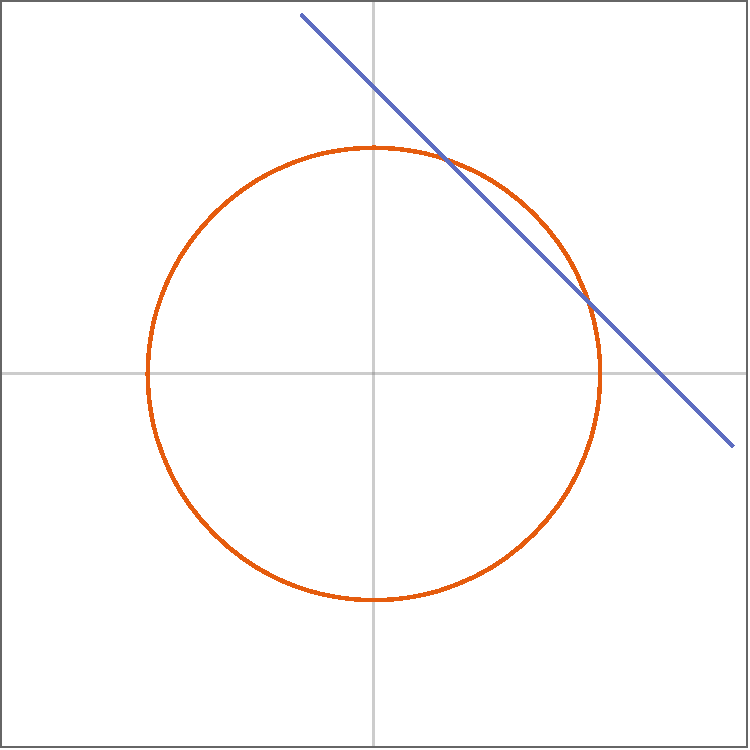
\includegraphics[width=\textwidth]{surfacesIn2D}
                \end{subfigure}%
                ~
                \begin{subfigure}[b]{0.5\textwidth}
                    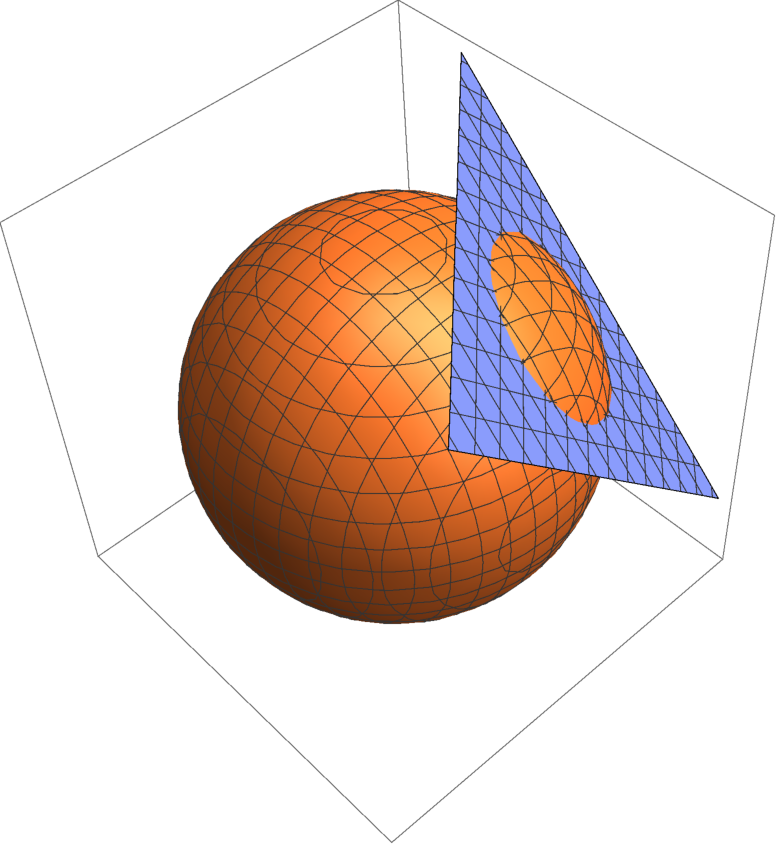
\includegraphics[width=\textwidth]{surfacesIn3D}
                \end{subfigure}
                \caption{The $\sum {n_i} = k$ and $\sum n_i^2 = k + \lambda$ surfaces in two and three dimensions.}
                \label{general:figure:surfaces}
            \end{figure}
                
            \begin{theorem}
                \label{general:theorem:limits}
                If $M$ is a $(Q,k)$-difference multiset then
                \begin{equation}
                    \forall q \in Q \colon \frac{k-(v-1)\sqrt k}{v} \leq n(q,M) \leq \frac{k+(v-1)\sqrt k}{v}
                \end{equation}
            \end{theorem}
            
            \begin{proof}
                Take \eqref{apparatus:eq:system} for the identity element and \eqref{apparatus:eq:ni} as constraints.
                
                \begin{equation}
                    \begin{cases}
                        \sum {n_i} = k \\
                        \sum (n_i(n_{i}-1)) = \lambda
                    \end{cases}
                \end{equation}
                
                Let's optimize $n_q$ respecting the constraints. We can add the first equation to the other to simplify the latter expression and let's also put all the terms on one side as follows.
                
                \begin{equation}
                    \begin{cases}
                        k - \sum {n_i} = 0 \\
                        k + \lambda - \sum n_i^2 = 0
                    \end{cases}
                \end{equation}
                
                We may now use a common optimization technique -- Lagrange multipliers to obtain the maximum and minimum of $n_q$ honoring the constraints by using the following Lagrange function (note that Lagranage multipliers $\lambda_1$ and $\lambda_2$ are notated per tradition and have nothing in common with the parameter $\lambda$).
                
                \begin{equation}
                    \mathcal L = n_q - \lambda_1 (k - \sum n_i) - \lambda_2 (k + \lambda - \sum n_i^2)
                \end{equation}
                
                This gives the stated boundaries for any $n_q$ in a difference multiset. The optimization calculations are not included as those are tedious and in no way novel.
            \end{proof}
        
            Theorem \ref{general:theorem:limits} might appear uninspiring at first but it greatly reduces the amount of options for every $n_q$. This simplification is a crucial stepping stone in making decent computer searches possible which allowed us to discover patterns that lead to results presented in this paper.
                
            \begin{figure}
                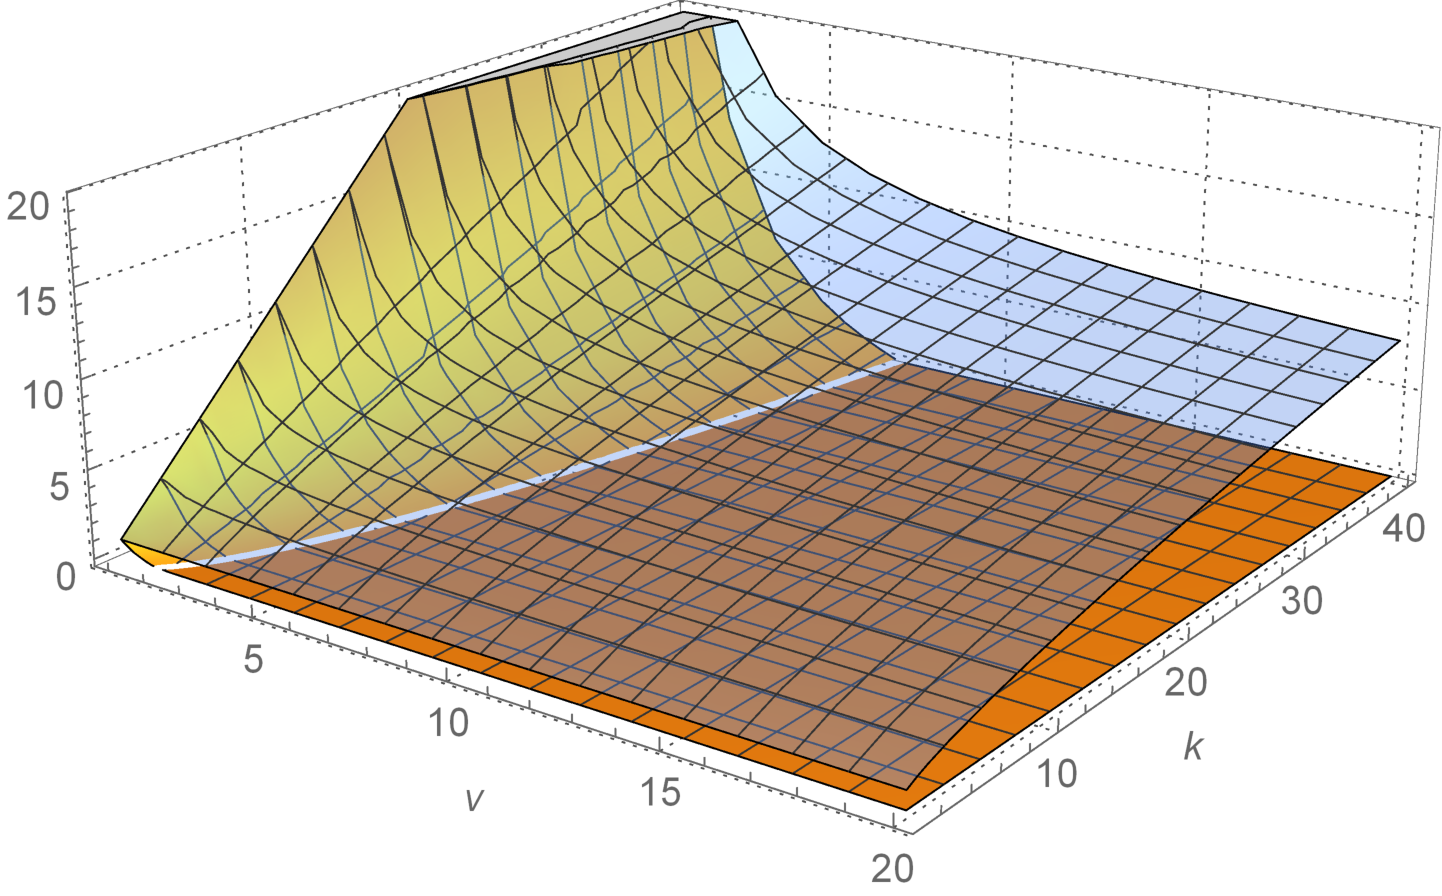
\includegraphics[width=\textwidth]{boundingSurfaces}
                \caption{Lower and upper limits for the values of $n_q$ with respect to $v$ and $k$.}
                \label{general:figure:limits}
            \end{figure}
            
        \subsection{A universal regular construction}
            Based on particular results discussed further, we have discovered a construction that works whenever $k$ is close to a multiple of $v$.
            
            \begin{theorem}
                \label{regular:theorem:regular}
                $(Q,k)$-difference multiset exists if $v \mid \sqrt k$ or $\sqrt k \equiv \pm 1 \mod v$ and it's digressions are 
                    \begin{itemize}
                        \item If $\sqrt k \equiv 1 \mod v$ then $d_i = v-1$ for any element $i$ and $d_{j \neq i} = -1$ for the other elements.
                        \item If $\sqrt k \equiv -1 \mod v$ then $d_i =1-v$ for any element $i$ and $d_{j \neq i} = 1$ for the other elements.
                        \item Both of the above if $v \mid \sqrt k$.
                    \end{itemize}
            \end{theorem}
            
            \begin{proof}
                The conditions in theorem guarantees the multiplicities to be integers. All that is left is to demonstrate that they actually make up a difference multiset and we will do that using our main equations in terms of digressions.
                
                Considering \eqref{apparatus:eq:dsystem} for non-identity elements we can notice that a any particular multiplicity will be involved in two of the products---once as $i$ and once as $i+q$ (but not both at the same time as we consider non-identity $q$ now). Other $v-2$ products are destined to contain other multiplicities solely which leads us to true equation.
                
                \begin{equation}
                    \sum d_i d_{i+q} = -2(v-1) + (v-2) = -v
                \end{equation}

                In case we're dealing with a loop, we must consider the case of $q$ being the identity which is also shown to be true.
                
                \begin{equation}
                    \sum d_i^2  = \left( \pm (v-1) \right)^2 + (v-1) \left( \mp 1 \right)^2 = v^2 - v
                \end{equation}
            
                It is straightforward to check that \eqref{apparatus:eq:di} turns out true as well.
            \end{proof}
        
        \subsection{Difference multisets for cyclic groups of even size}
            For loops we can rewrite \eqref{apparatus:eq:dmatrixform}:
            
            \begin{equation}
                C g' = \bf v'
            \end{equation}\
            where $g'_q: i \rightarrow (d_i d_q)$ and $v'_q = v(v\delta_{q0}-1)$.
            
            As the operation of $g'$ is pretty trivial, we can write it even more nicely:
            
            \begin{equation}
                D d = \bf v'
            \end{equation}
                where $D_{ij} = d_{C_{ij}}$ (i.e. replace elements in Cayley table with their digressions) and $d_q = d_q$.

            As the title suggests, we will be dealing with cyclic groups in this section. That's because of the nice Cayley table they possess. The Cayley table of cyclic groups of size $v$ takes the following form:
            
            \begin{equation}
                \label{general:eq:anticirculant_matrix}
                \begin{pmatrix}
                    0 & 1 & 2 & \cdots & v-2 & v-1 \\ 
                    1 & 2 & 3 & \cdots & v-1 & 0 \\
                    \vdots & \vdots & \vdots & \ddots & \vdots & \vdots \\
                    v-2 & v-1 & 0 & \cdots & v-4 & v-3 \\
                    v-1 & 0 & 1 & \cdots & v-3 & v-2
                \end{pmatrix}
            \end{equation}
	
            This is a special case of Hankel matrix sometimes called \emph{anticirculant matrix}. The structure of the corresponding $D$ will be the same.
            
            \subsubsection{Solving equations with anticirculant matrices}
            \label{general:sec:anticirculant}
                We weren't able to track down a source dealing with matrices like \eqref{general:eq:anticirculant_matrix}, however it's fairly straightforward to apply the same methods as with circulant matrices \cite{wiki:circulant_matrix}.
                
                Let's consider the equation $Ax=b$ with an anticirculant $v \times v$ matrix
                \begin{equation}
                    A =
                    \begin{pmatrix}
                        a_0 & a_1 & a_2 & \cdots & a_{v-1} \\ 
                        a_1 & a_2 & a_3 & \cdots & a_0 \\
                        a_2 & a_3 & a_4 & \cdots & a_1 \\
                        \vdots & \vdots & \vdots & \ddots & \vdots \\
                    \end{pmatrix}
                \end{equation}\
                and a vector $b=(b_0, b_1, b_2, \vdots)^T$. 
                
                Denote $a=(a_1,\ldots,a_{v-1})$. We can now express the equation row by row (please consider indices $\mod v$):
                \begin{equation}
                    b_j = \sum_{k=0}^{v-1} a_{j+k} x_k
                \end{equation}
                
                Apply discrete Fourier transform:
                \begin{equation}
                    \mathcal{F} (b)_m = \sum_{j=0}^{v-1} b_j \exp(-2\pi i \frac{jm}v )
                \end{equation}
                
                Insert $b_j$ obtaining
                \begin{equation}
                \begin{split}
                    \mathcal{F} (b)_m
                    &= \sum_{j=0}^{v-1} \sum_{k=0}^{v-1} a_{j+k} x_k \exp(-2\pi i \frac{jm}v) \\
                    &= \sum_{j=0}^{v-1} \sum_{k=0}^{v-1} x_k \exp(2\pi i \frac{km}v) a_{j+k} \exp(-2\pi i \frac{(j+k)m}v)  \\
                    &= \sum_{k=0}^{v-1} x_k \exp(2\pi i \frac{km}v) \sum_{j'=k}^{v+k-1} a_{j'} \exp(-2\pi i \frac{j'm}v)
                \end{split}
                \end{equation}
                
                Looking at the inner sum we should note that not only we take indices $\mod v$ but the $j'$ in the exponent can be taken $\mod v$ as well. Let's use $j'' = j' \mod v$.
                \begin{equation}
                    \sum_{j'=k}^{v+k-1} a_{j'} \exp(-2\pi i \frac{j'm}v) = 
                    \sum_{j''=0}^{v-1} a_{j''} \exp(-2\pi i \frac{j''m}v) = \mathcal{F}(a)_m
                \end{equation}
                
                We can now finish the transformation:
                \begin{equation}
                \begin{split}
                    \mathcal{F} (b)_m
                    &= \sum_{k=0}^{v-1} x_k \exp(2\pi i \frac{km}v) \mathcal{F}(a)_m \\
                    &= \mathcal{F}(a)_m (\sum_{k=0}^{v-1} x^*_k \exp(-2\pi i \frac{km}v))^* \\
                    &= \mathcal{F}(a)_m \mathcal{F}^*(x^*)_m 
                    = v \mathcal{F}(a)_m \mathcal{F}^{-1}(x)_m
                \end{split}
                \end{equation}
                
                The final form (exploiting the Fourier transform property $\mathcal{F}^{-1}(x) = \mathcal{F}^*(x^*)/v$) was included for completeness as it allows to explicitly express $x = \mathcal{F} \left(\frac1v \frac{\mathcal{F}(b)}{\mathcal{F}(a)} \right)$. However, we will use $\mathcal{F} (b)_m = \mathcal{F}(a)_m \mathcal{F}^*(x^*)_m$.
            
            \subsection{Solving the digression equation}
                The $D$ and $d$ in equation $Dd=\bf v'$ is linked in the same way as $A$ and $a$ in subsection \ref{general:sec:anticirculant}. The image of $Dd=\bf v'$ is
                
                \begin{equation}
                    \mathcal{F} ({\bf v'})_m = \mathcal{F}(d)_m \mathcal{F^*}(d^*)_m
                \end{equation}

                As we are only interested in real $d$, we can even simplify it to
                
                \begin{equation}
                    \label{general:eq:dfourier}
                    \mathcal{F} ({\bf v'})_m = \mathcal{F}(d)_m \mathcal{F^*}(d)_m = |\mathcal{F}(d)_m|^2
                \end{equation}
                
                Putting the identity first we have ${\bf v'} = (v^2-v, -v, -v, \ldots)$ and $\mathcal{F}({\bf v'}) = (0,v^2,v^2,\ldots)$. Thus \eqref{general:eq:dfourier} becomes
                \begin{equation}
                    \left| \sum_{j=0}^{v-1} d_j \exp(-2\pi i \frac{jm}v) \right| = v (1-\delta_{m0})
                \end{equation}

                Note that for any $m | v$
                \begin{equation}
                    \label{general:eq:split_fourier}
                    \left| \sum_{j=0}^{v-1} d_j e^{\frac{-2\pi i m j}v} \right|
                    = \left| \sum_{j=0}^{v/m-1} \sum_{k=0}^{m-1}  d_{j+kv/m} e^{\frac{-2\pi i m j}v} \right|
                    =v (1-\delta_{m0})
                \end{equation}\
                as 
                \begin{equation}
                    e^{\frac{-2\pi i m (j+kv/m)}v} = e^{\frac{-2\pi i m j}v} e^{-2\pi i k} = e^{\frac{-2\pi i m j}v}
                \end{equation}
                
                \begin{theorem}
                    \label{general:theorem:even_cyclic}
                    In cyclic groups of even cardinality $\sum_{k=0}^{v/2-1} d_{2k} = \pm \frac v2$ and $\sum_{k=0}^{v/2-1} d_{2k+1} = \mp \frac v2$.
                \end{theorem}
                \begin{proof}
                    Take \eqref{general:eq:split_fourier} for $m=v/2$
                    \begin{equation}
                        \left| \sum_{k=0}^{v/2-1} d_{2k} - \sum_{k=0}^{v/2-1} d_{2k+1} \right| = v
                    \end{equation}
                    
                    We've split $d$ in half and got that total of one half is by $v$ larger than the total of the other half. The statement of the theorem follows as soon as we remember the grand total $\sum d_i = 0$.
                \end{proof}
            
	\section{Smallest difference multisets}
        Bulk of our results concern difference multisets with small $v$. But let's start from zero.
	
		\subsection{Trivial cases}
			We should get these out of the way first. While not interesting on their own, these cases may turn out useful when looking for patterns and drawing parallels with other research.
			
			If $v=1$ (the trivial group) there is a $(\set{0},k)$-difference multiset for any value of $k$: just take the identity $k$ times and all the rules will be satisfied.
			
			The cases of $k=0$ and $k=1$ is also universally good. For any quasigroup $Q$ you can take no elements to make a $(Q,0)$-difference multiset or a single element once to form a $(Q,1)$-difference multiset. In both of these cases $\lambda=0$ i.e. the difference multiset produces every element of $Q$ exactly $0$ times.
			
			An exception to the above arises when we take the empty quasigroup combined with $k=1$---one can't take a single element from it so there is no $(\set{}, 1)$-difference multiset unfourtunately.
			
		\subsection{The two-element group}
			There is only one quasigroup with two elements which also happens to be a commutative group. Let's take it in the form $\mathbb Z_2$.
		
			This case was solved by Buratti \cite{buratti1999old}. We will provide a solution for this case for completeness of low-parameter cases.
			
			\begin{theorem}
				$(\mathbb Z_2,k)$-difference multiset exists whenever $k$ is a perfect square. In that case $n_0 = \frac{k \pm \sqrt k}{2}$ and $n_1 = \frac{k \mp \sqrt k}{2}$.
			\end{theorem}
			\begin{proof}
                Theorem \ref{general:theorem:even_cyclic} provides $d_0 = \pm 1$ and $d_1 = \mp -1$.
                
                Notice that these $d_i$ produce integer $n_i = \frac{k + d_i \sqrt k}2$ whenever $k$ is a square.
			\end{proof}
			
			\begin{remark}
                We did not bother to discuss the case of non-square $k$ as it is proven in \cite{arasu2005cyclic} (see theorem 2.3) that there can only be a difference multiset over abelian group with an even $v=|G|$ if the $k$ is square.
			\end{remark}

	\section{Difference multisets over the three element group}
		There is only one group of three elements. Let's take it in form of $\mathbb Z_3$. What must the $k$ be for $(\mathbb Z_3,k)$-difference multiset to exist? What are these difference multisets and how many of them are there for a particular value of $k$?
		
		To answer these questions we shall write down \eqref{apparatus:eq:system} for a non-identity element and combine it with \eqref{apparatus:eq:ni} and \eqref{apparatus:eq:parameters} to form a system of equations.
		
		\begin{equation}
			\label{v3:eq:constraints}
			\begin{cases}
				3\lambda = k(k-1) \\
				\sum n_i = k \\
				\sum n_i n_{i+1} = \lambda
			\end{cases}
		\end{equation}
		
		We may now combine the equations to discover a relation between multiplicities of elements.
		
		\begin{theorem}
			\label{v3:theorem:relations}
			Multiplicities of different $(\mathbb Z_3,k)$-difference multiset elements $i$ un $j$ are related via
			\begin{equation}
				\label{v3:eq:relations}
				n_{i\neq j} = \frac{k-n_j \pm \sqrt{\frac{4k-(k-3n_j)^2}{3}}}{2}
			\end{equation}
		\end{theorem}
		
		\begin{proof}
			Take any element $\gamma \in \mathbb Z_3$ and assign $c = n_\gamma$. Let's use $\alpha$ and $\beta$ to name the remaining elements of $\mathbb Z_3$. The system \eqref{v3:eq:constraints} can now be rewritten:
			\begin{equation}
				\begin{cases}
					n_\alpha + n_\beta = k - c \\
					n_\alpha n_\beta + c (n_\alpha + n_\beta)  = \lambda 
				\end{cases}
			\end{equation}
			
			Substitute $k'=k-c$ and $\lambda' = \lambda + c^2-kc$ to obtain
			
			\begin{equation}
				\begin{cases}
					n_\alpha + n_\beta = k' \\
					n_\alpha n_\beta = \lambda'
				\end{cases}
			\end{equation}
			
			Eliminating $n_\beta$ we arrive at a quadratic equation that is solved into
			
			\begin{equation}
				n_\alpha = \frac{k' \pm \sqrt{k'^2-4\lambda'}}{2}
			\end{equation}
			
			Undo the substitutions and you're done.
		\end{proof}
		
		Considering the multiplicities in form of $n_i = \frac{k+\Delta_i}{3}$, we can restate \eqref{v3:eq:relations} into the following.
	
		\begin{equation}
			\label{v3:eq:relations_delta}
			n_{i\neq j} = \frac{k-n_j \pm \sqrt{\frac{4k-\Delta_j^2}{3}}}{2}
		\end{equation}
		
		The rest of analysis focuses on the $\Delta_i$ and it's effect on the above equation. The behaviour of expression under the root is tied to a topic in number theory called Löschian numbers \cite{oeisA003136}. These numbers make an appearance in a variety of fields (see comments in \cite{oeisA003136}).
		
		\begin{definition}
			\label{v3:def:loeshian}
			Number $k$ is called a Löschian number if $\exists a,b \in \mathbb Z \colon a^2+ab+b^2=k$.
		\end{definition}
		
		For our purposes (to eliminate unnecessary symmetries) we will only consider $a,b$ such that $a \geq b \geq 0$. This, however, doesn't change the scope of Löschian numbers.
		
		\begin{lemma}
			\label{v3:lemma:loeschian}
			For any Löschian number $k$ we can find $a,b \in \mathbb Z$ such that $a^2+ab+b^2=k$ and $a \geq b \geq 0$.
		\end{lemma}
		
		\begin{proof}
			As $k$ is a Löschian number there are $a',b' \colon a'^2+a'b'+b'^2=k$. We can construct $a,b$ such that $a^2+ab+b^2=k$ and $a \geq b \geq 0$ as follows:
			\begin{itemize}
				\item If $a' \geq 0$ and $b' \geq 0$ just take $a=a'$ and $b=b'$ or swap them if $a'<b'$.
				\item If $a'<0,b'<0$ take $a'=-a,b'=-b$ or swap them if $a'>b'$.
				\item If $ab<0$ take either $a'=|a|, b'=|a+b|$ or $a'=|a+b|, b'=|b|$. Swap places as necessary to ensure $a \geq b \geq 0$.
			\end{itemize}
		\end{proof}
		
		Having introduced the term, we may now introduce the promised link.
		
		\begin{lemma}
			\label{v3:lemma:square}
			There exists a $\Delta$ that makes $\frac{4k-\Delta^2}{3}$ a perfect square iff $k$ is Löschian number.
			
			$\Delta$ values that does the job are $\pm (2a+b), \pm (a+2b), \pm (a-b)$, where $a,b$ are such that $a \geq b \geq 0$ and $a^2+ab+b^2=k$. There is no other $\Delta$ that makes $\frac{4k-\Delta^2}{3}$ into square.
		\end{lemma}
		
		\begin{proof}
			For a Löschian number $k=a^2+ab+b^2$ take $\Delta$ equal to $\pm (2a+b)$, $\pm (a+2b)$ or $\pm (a-b)$ and obtain the value of expression in question to be $b^2$, $a^2$ or $(a+b)^2$ which are clearly squares.
			
			On the other hand, if $\frac{4k-\Delta^2}{3}$ is square, assign:
			\begin{equation}
				z^2 = \frac{4k-\Delta^2}{3}
			\end{equation}
			
			Rewrite
			\begin{equation}
				\frac{3z^2 + \Delta^2}{4} = k
			\end{equation}
			
			Noticing that $4$ divides $3z^2 + \Delta^2$ we can conclude that $z$ and $\Delta$ are of the same parity (because $z^2 \equiv \Delta^2 \mod 4$). Thus $2$ divides both $\Delta-z$ and $\Delta+z$.
			
			We can now find integers $a,b$ such that $a \geq b \geq 0$ and $a^2+ab+b^2=k$ (thus $k$ is a Löschian number) and the $\Delta$ can be expressed in one of the expressions stated in lemma.
			
			\begin{itemize}
				\item If $z \geq \Delta$ take $a=\frac{z+\Delta}{2}$ and $b=\frac{z-\Delta}{2}$. Then $a-b=\Delta$.
				\item If $\Delta \geq z \geq \frac \Delta 3$ take $a=z$ and $b=\frac{\Delta-z}{2}$. Then $a+2b=\Delta$.
				\item If $\frac \Delta 3 \geq z$ take $a=\frac{\Delta-z}{2}$ and $b=z$. Then $2a+b=\Delta$.
			\end{itemize}
		\end{proof}
		
		Let's introduce the following notation for the three values used in lemma \ref{v3:lemma:square}. The rest can be expressed as $-\Delta_i$:
		\begin{equation}
			\label{v3:eq:deltas}
			\Delta_\alpha = 2a+b, \Delta_\beta = -a-2b, \Delta_\gamma = -a+b
		\end{equation}
		
		These $\Delta_i$ will be used in the following theorem and $\alpha$, $\beta$ and $\gamma$ are labels that, as before, we use to label the elements of $\mathbb Z_3$ in arbitrary order. We can now state our main result which is both construction and existence criterion for $(\mathbb Z_3,k)$-difference multisets.
		
		\begin{theorem}
			\label{v3:theorem:loeschian}
			For every pair $a,b \in \mathbb Z$ such that $k=a^2+ab+b^2$ and $a \geq b \geq 0$ there are exactly $-(k+1) \mod 3$ (up to automorphisms) $(\mathbb Z_3,k)$-difference multisets and the multiplicities of their elements are
			
			\begin{itemize}
				\item $n_i=\frac{k+\Delta_i}{3}$ for one and $n_i=\frac{k-\Delta_i}{3}$ for the other if $3 \mid k$.
				\item $n_i=\frac{k+\Delta_i}{3}$ if $3 \nmid k$ un $b-a \equiv 1 \mod 3$.
				\item $n_i=\frac{k-\Delta_i}{3}$ if $3 \nmid k$ un $a-b \equiv 1 \mod 3$.
			\end{itemize}
		\end{theorem}
		
		\begin{proof}
			According to lemma \ref{v3:lemma:square}, the expression \eqref{v3:eq:relations_delta} will equal integer only if $k$ is a Löschian number and $\Delta_j$ is one of the listed on \eqref{v3:eq:deltas} or a negative of that.
			
			Insert the constructions listed in \eqref{v3:theorem:loeschian} into \eqref{v3:eq:relations} to check that these are indeed multiplicities that make up a difference multiset if the numbers are whole. One can also check that using $\Delta_\alpha$ to construct one of the multiplicities you will notice $\Delta_\beta$ and $\Delta_\gamma$ used for the others and the same is true in any order.
			
			Considering remainders one may check the following:
			\begin{itemize}
				\item If $a \equiv b \mod 3$ then $3 \mid k$ and all the multiplicities in both the constructions $n_i=\frac{k+\Delta_i}{3}$ and $n_i=\frac{k-\Delta_i}{3}$ are integers.
				\item If $a \equiv b-1 \mod 3$ then $k \equiv 1 \mod 3$ and only the multiplicities constructed by $n_i=\frac{k+\Delta_i}{3}$ are all integer.
				\item If $a \equiv b+1 \mod 3$ then $k \equiv 1 \mod 3$ and only the multiplicities constructed by $n_i=\frac{k-\Delta_i}{3}$ are all integer.
			\end{itemize}
		\end{proof}

		\begin{remark}
			Allowing $a,b$ such that $a \geq b \geq 0$ wouldn't hold, we'd obtain the same $\Delta_\alpha, \Delta_\beta, \Delta_\gamma$ in different order thus making the same difference multisets again (up to automorphism). This constraint is intended to exclude such symmetries.
			Different $a \geq b \geq 0$ pairs with $a^2+ab+b^2=k$ will lead to different value of $a-b$ and thus all the constructions mentioned in \ref{v3:theorem:loeschian} will be distinct. Consequently the number of $(\mathbb Z_3,k)$ will be proportional to number of unique $a,b$ pairs (respecting constraints) and the coefficient of proportionality is $-(k+1) \mod 3$.
		\end{remark}
		
		\subsection{Estimating numbers}
			Despite our effort, the exact number of solutions is still elusive. This aspect is now reduced to a number-theoretic question -- how many unique solutions are there for $k=a^2+ab+b^2$ such that $a\geq b\geq 0$.
		
			The number of solutions without the constraint is known \cite{marmon2005hexagonal}. Denote
			\begin{equation}
				k=3^\alpha p_1^{\alpha_1}p_2^{\alpha_2}\ldots q_1^{\beta_1}q_2^{\beta_2}\ldots
			\end{equation}\
			
			where $p_i$ are primes such that $p_i \equiv 1 \mod 3$ and $q_i$ are primes such that $q_i \equiv 2 \mod 3$. If any of the $\beta_i$ are odd, there are no integer solutions to $k=a^2+ab+b^2$. But if all of $\beta_i$ are even, the number of solutions is $6\prod (\alpha_i +1)$.
			
			It is hypothesised \cite{nair2004elementary} that the number of solutions (if every $\beta_i$ is even) having $a \geq b \geq 0$ is $1/2 + \prod (\alpha_i +1)/2$ if all the $\alpha_i$ are even and $\prod (\alpha_i +1)/2$ otherwise. We checked this to be true for a thousand Löschian numbers. However, for most of the Löschian numbers this remains unchecked.
	
		\subsection{Other structures of the same size}
			As mentioned in the opening sections, one might also consider $(\mathbb Z_3,k)$-sum multisets where the elements of $\mathbb Z_3$ must be produced as the sums of elements. This turns out to be a simple case.

			Similarly to \eqref{apparatus:eq:system} we start by writing down the ways to obtain each of the elements and requiring them to be equal ($\forall j \in \mathbb Z_3 \lambda = \sum (n_i(n_{i-j}-\delta_{i,i-j}))$). Adding the $\sum n_i = k$ and using $3\lambda = k(k-1)$ we may form a system of equations.
			
			\begin{equation}
				\label{v3:other:eq:system}
				\begin{cases}
					n_0 (n_0-1) + 2 n_1 n_2 = \frac{k(k-1)}{3} \\
					n_1 (n_1-1) + 2 n_2 n_0 = \frac{k(k-1)}{3} \\
					n_2 (n_2-1) + 2 n_0 n_1 = \frac{k(k-1)}{3} \\
					n_0 + n_1 + n_2 = k
				\end{cases}
			\end{equation}
	
			It can be noticed with ease that \eqref{v3:other:eq:system} possesses symmetry with respect to all the elements of $\mathbb Z_3$. Besides this system can easily be solved explicitly -- valid multisets of $n_i$ are $\set{\frac k 3, \frac k 3, \frac k 3}$ and $\set{\frac{k-1}{3}, \frac{k-1}{3}, \frac{k+2}{3}}$.
			
			So, we can conclude that there can be at most one (up to automorphisms) $(\mathbb Z_3, k)$-sum multiset for a given value $k$. Specifically there is one if $3 \mid k$ or $k \equiv 1 \mod 3$ and the multiplicities of elements are $\set{\frac k 3, \frac k 3, \frac k 3}$ and $\set{\frac{k-1}{3}, \frac{k-1}{3}, \frac{k+2}{3}}$ respectively. And there are none if $k \equiv 2 \mod 3$ which eerily reminds of the situations with difference multisets.
			
			Recall remark \ref{dms:remark:abelian}. If we consider any other quasigroup of order 3, it turns out that in every case the difference multisets and sum multisets give raise to either system \eqref{v3:eq:constraints} or the system \eqref{v3:other:eq:system}. There are only 5 quasigroups of order 3 so this can be checked on a case by case basis. We have thus solved the problem for every quasigroup of size 3.
	
    \section{Other decent cases}
        \subsection{Difference multisets over $\mathbb Z_2 \times \mathbb Z_2$}
            Let us now consider group $\mathbb Z_2 \times \mathbb Z_2$. In this case our apparatus gives raise to the following system of equations.
            
            \begin{equation}
                \label{v4:eq:constraints}
                \begin{cases}
                    \sum d_i^2 = 12 \\
                    \sum d_i = 0 \\
                    d_{00} d_{01} + d_{10} d_{11} = -2 \\
                    d_{00} d_{10} + d_{01} d_{11} = -2 \\
                    d_{00} d_{11} + d_{10} d_{01} = -2
                \end{cases}
            \end{equation}
            
            \begin{theorem}
                \label{v4:theorem:z2z2}
                $(\mathbb Z_2 \times \mathbb Z_2, k)$--difference multisets exist iff $\sqrt k \equiv 0 \mod 4$ or $\sqrt k \equiv \pm 1 \mod 4$. The multiplicities are:
                \begin{itemize}
                    \item $\frac{k + 3 \sqrt k}{4}$ for one element and $\frac{k - \sqrt k}{4}$ for the other three if $\sqrt k \equiv 1 \mod 4$.
                    \item $\frac{k - 3 \sqrt k}{4}$ for one element and $\frac{k + \sqrt k}{4}$ for the other three if $\sqrt k \equiv -1 \mod 4$.
                    \item $\frac{k \pm 3 \sqrt k}{4}$ for one element and $\frac{k \mp \sqrt k}{4}$ for the other three if $4 \mid \sqrt k$.
                \end{itemize}
            \end{theorem}
            
            \begin{proof}
                Solve \eqref{v4:eq:constraints} to find eight solutions each having one $d_i = \pm 3$ and the rest $d_{j \neq i} = \mp 1$.
                
                Notice that these numbers yield integer $n_i = \frac{k+d_i \sqrt k}4$ values in and only in the cases described in theorem.
            \end{proof}
	
		\subsection{Difference multisets over $\mathbb Z_4$}
			It is easy to check that all of the solutions stated in theorem \ref{v4:theorem:z2z2} also work here, so it's clear that a solution exists if and only if $\sqrt k \in \mathbb Z$ and $\sqrt k \not\equiv 2 \mod 4$ (i.e. whenever $\lambda$ is even).
			
			\begin{figure}
				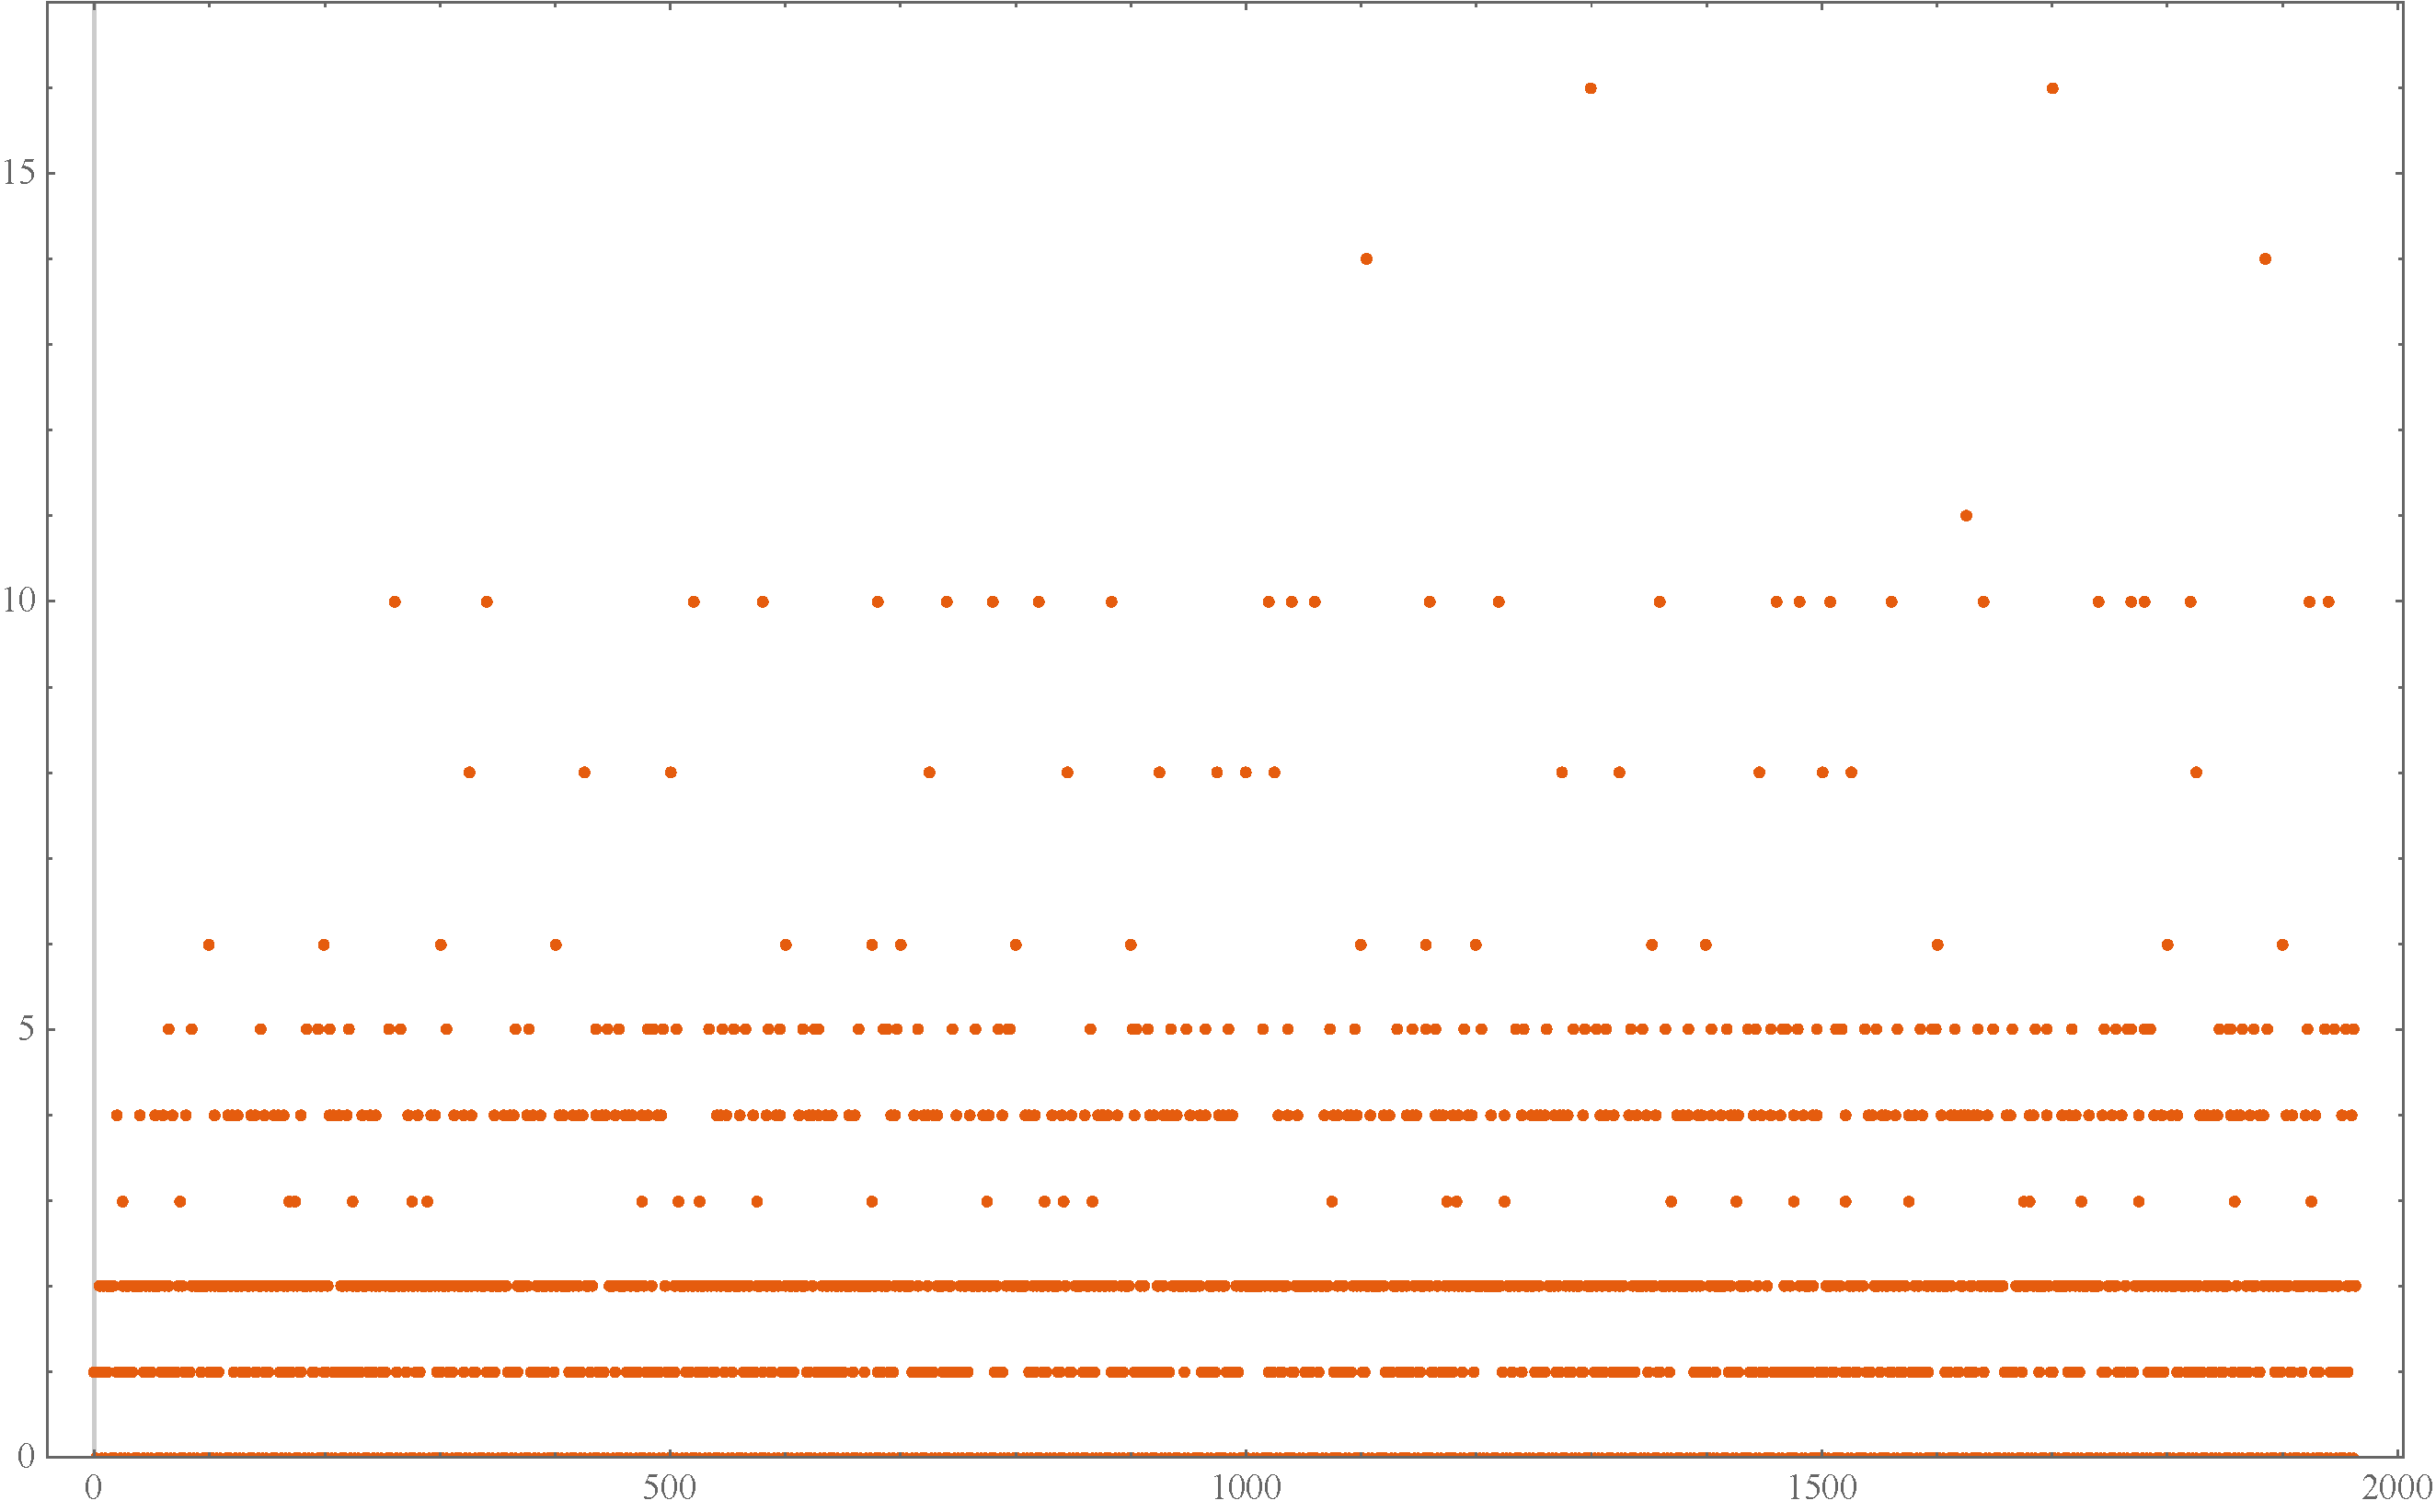
\includegraphics[width=\textwidth]{z4}
				\caption{Number of $(\mathbb Z_4, k)$-difference multisets (excluding automorphisms) with respect to $\sqrt k$.}
				\label{other:z4:figure:results}
			\end{figure}
			
			However, our numerical experiments show that the one or two solutions given in \ref{v4:theorem:z2z2} are not the only ones working for this group. Smallest of the solutions not constructed in theorem \ref{v4:theorem:z2z2} arises for $k=25$ where a difference multiset can have multiplicities not only $\set{5,5,5,10}$, but also $\set{3,6,7,9}$. 

			The numbers of solutions for $k$ not too large are depicted in figure \ref{other:z4:figure:results}. One can observe that with $k$ increasing we have cases of more and more solutions that can't be explained by the known construction.
			
		\subsection{Difference multisets over $\mathbb Z_2 \times \mathbb Z_2 \times \mathbb Z_2$}
			\begin{theorem}
				A $(\mathbb Z_2 \times \mathbb Z_2 \times \mathbb Z_2, k)$-difference multiset can only be constructed by taking multiplicities $n_i$ with the following digressions:
				\begin{itemize}
					\item If $\sqrt k \equiv -1 \mod 8$ take $d_i=-7$ for any $i$ and $d_j=1$ for other $j\neq i$.
					\item If $\sqrt k \equiv 1 \mod 8$ take $d_i=7$ for any $i$ and $d_j=-1$ for other $j\neq i$.
					\item If $\sqrt k \equiv 0 \mod 8$ choose any element $i$ and three distinct elements $j_1,j_2,j_3$ such that $j_1+j_2+j_3=0$. Set $d_i=\pm 5$ and $d_{i+j_1}=d_{i+j_2}=d_{i+j_3}=\mp 3$ and let the other four $d_k = \pm 1$. Besides, both of the above solutions will work as well.
				\end{itemize}
			\end{theorem}
			
			\begin{proof}
				Write down \eqref{apparatus:eq:di} and \eqref{apparatus:eq:dsystem} for this case:
				
				\begin{equation}
					\begin{cases}
                        d_{000} + d_{001} + d_{010} + d_{011} + d_{100}  + d_{101}  + d_{110}  + d_{111} = 0 \\
                        d_{001}^2 + d_{010}^2 + d_{010}^2 + d_{011}^2 + d_{100}^2 + d_{101}^2 + d_{110}^2 + d_{111}^2 = 56 \\
                        d_{000} d_{001} + d_{010} d_{011} + d_{100} d_{101} +  d_{110} d_{111} = -4 \\
                        d_{000} d_{010} + d_{001} d_{011} + d_{100} d_{110} +  d_{101} d_{111} = -4 \\
                        d_{000} d_{011} + d_{001} d_{010} + d_{100} d_{111} +  d_{101} d_{110} = -4 \\
                        d_{000} d_{100} + d_{001} d_{101} + d_{010} d_{110} +  d_{011} d_{111} = -4 \\
                        d_{000} d_{101} +  d_{001} d_{100} + d_{010} d_{111} + d_{011} d_{110} = -4 \\
                        d_{000} d_{110} + d_{001} d_{111} + d_{010} d_{100} + d_{011} d_{101} = -4 \\
                        d_{000} d_{111} + d_{001} d_{110} + d_{010} d_{101} +  d_{011} d_{100} = -4
					\end{cases}
				\end{equation}
				
				Solve to obtain the given solutions and notice that they yield integer $n_i = \frac{k+d_i \sqrt k}8$ whenever $\sqrt k$ behaves as described in the cases of theorem.
			\end{proof}

	\section{Conclusions}
		Although this topic seems far from complete, we have reached multiple small breakthroughs in various directions.
		
		The case of difference multisets over $\mathbb Z_3$ (theorem \ref{v3:theorem:loeschian}) shows that not only the very trivial cases can be solved explicitly. Although it is not straightforward to generalize our methods for arbitrary $\mathbb Z_k$, solving the problem for an odd prime value of $k$ seems promising. Furthermore the discovered link to Löschian numbers might provide further insight for other difference multisets or even some new perspective on the topics now linked through Löschian numbers.
		
		The solved $\mathbb Z_2 \times \mathbb Z_2$ and $\mathbb Z_2 \times \mathbb Z_2 \times \mathbb Z_2$ is another promising direction. A new construction (theorem \ref{regular:theorem:regular}) was found generalizing ones of $\mathbb Z_2$ and $\mathbb Z_2 \times \mathbb Z_2$ and it feels a general solution for $G=\prod_{i=1}^{n} \mathbb Z_2$ should be in reach soon.
		
		And lastly, theorem \ref{general:theorem:limits} greatly narrows the space of options that has to be considered in computer searches thus allowing to inspect a wide range of difference multisets and draw conclusions through observations.

	\bibliographystyle{plain}
	\bibliography{difference_multisets} 
		
\end{document}
